\thispagestyle{duongvaotoanhocnone}
\pagestyle{duongvaotoanhoc}
\everymath{\color{duongvaotoanhoc}}
\graphicspath{{../duongvaotoanhoc/pic/}}
\blfootnote{$^1$\color{duongvaotoanhoc}Universit\'e Paris--Saclay.}
\begingroup
\AddToShipoutPicture*{\put(0,616){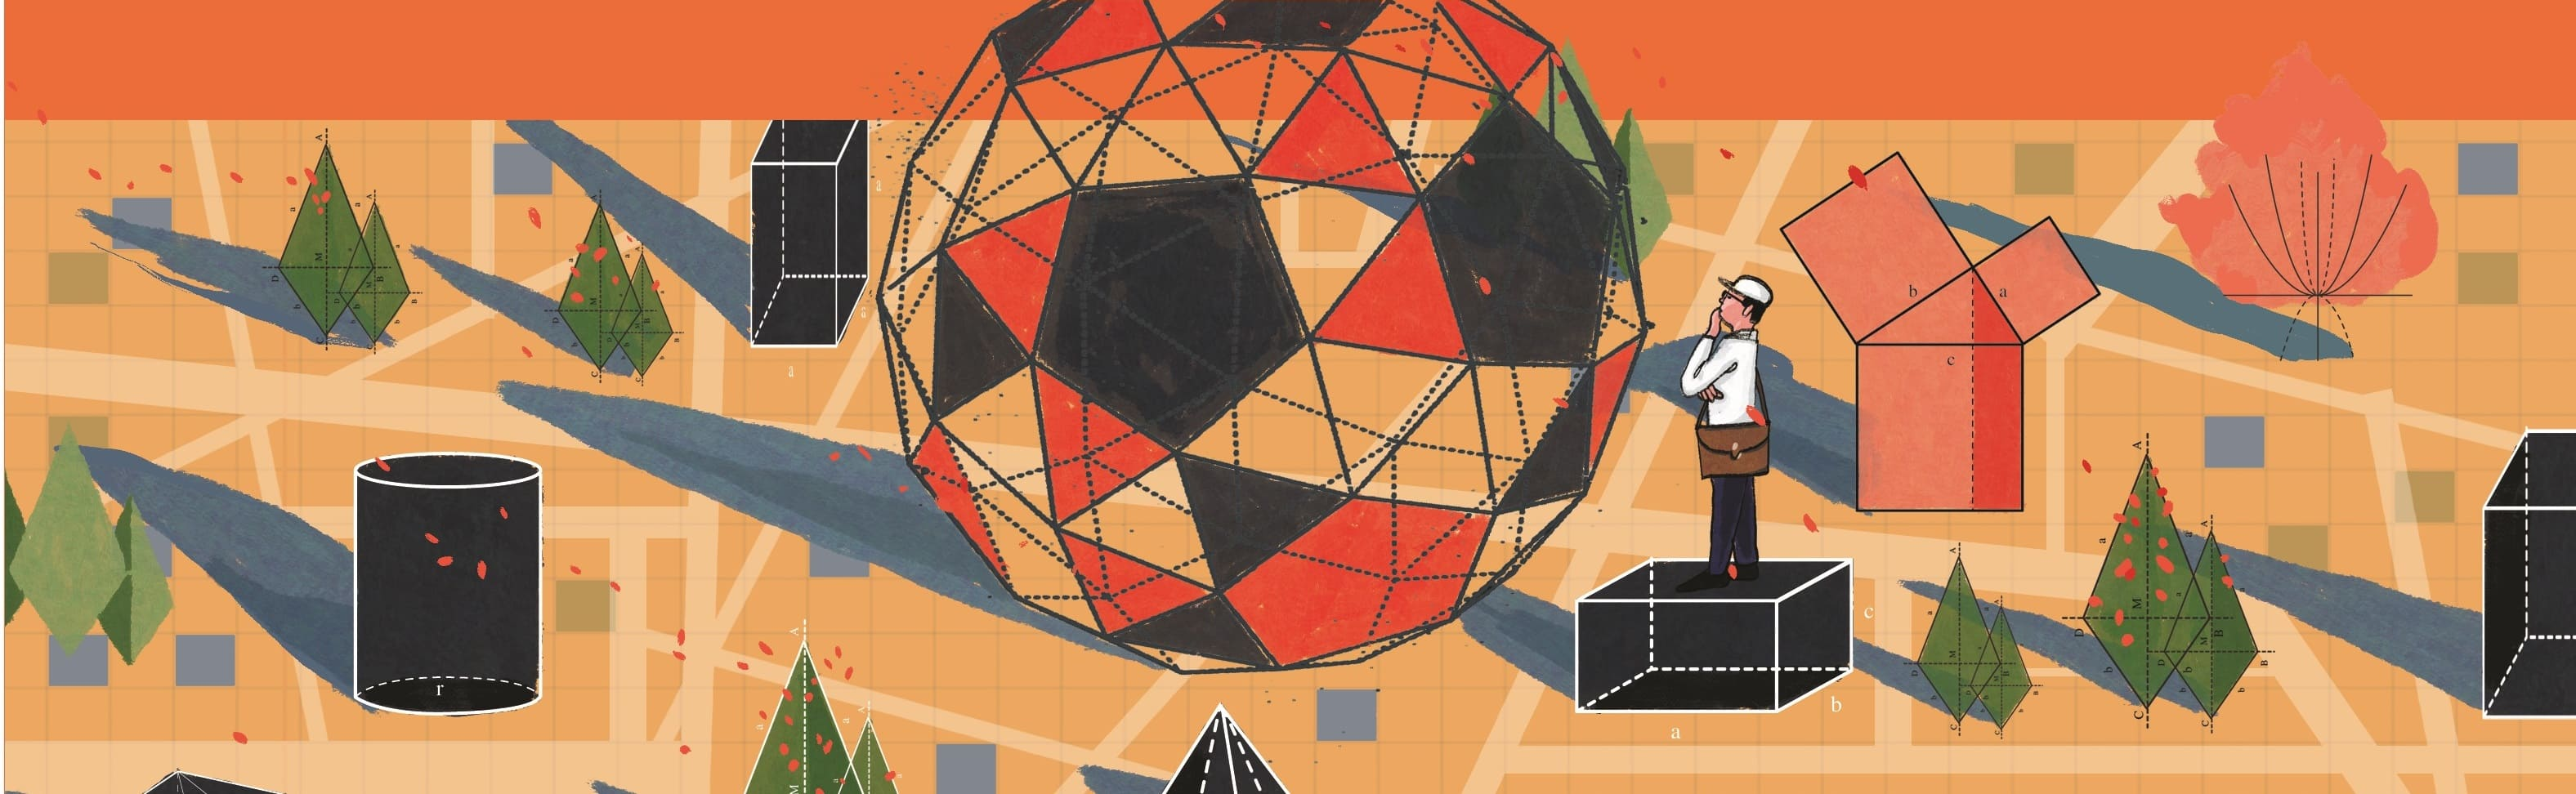
\includegraphics[width=19.3cm]{../bannerduongvao}}}
\AddToShipoutPicture*{\put(84,523){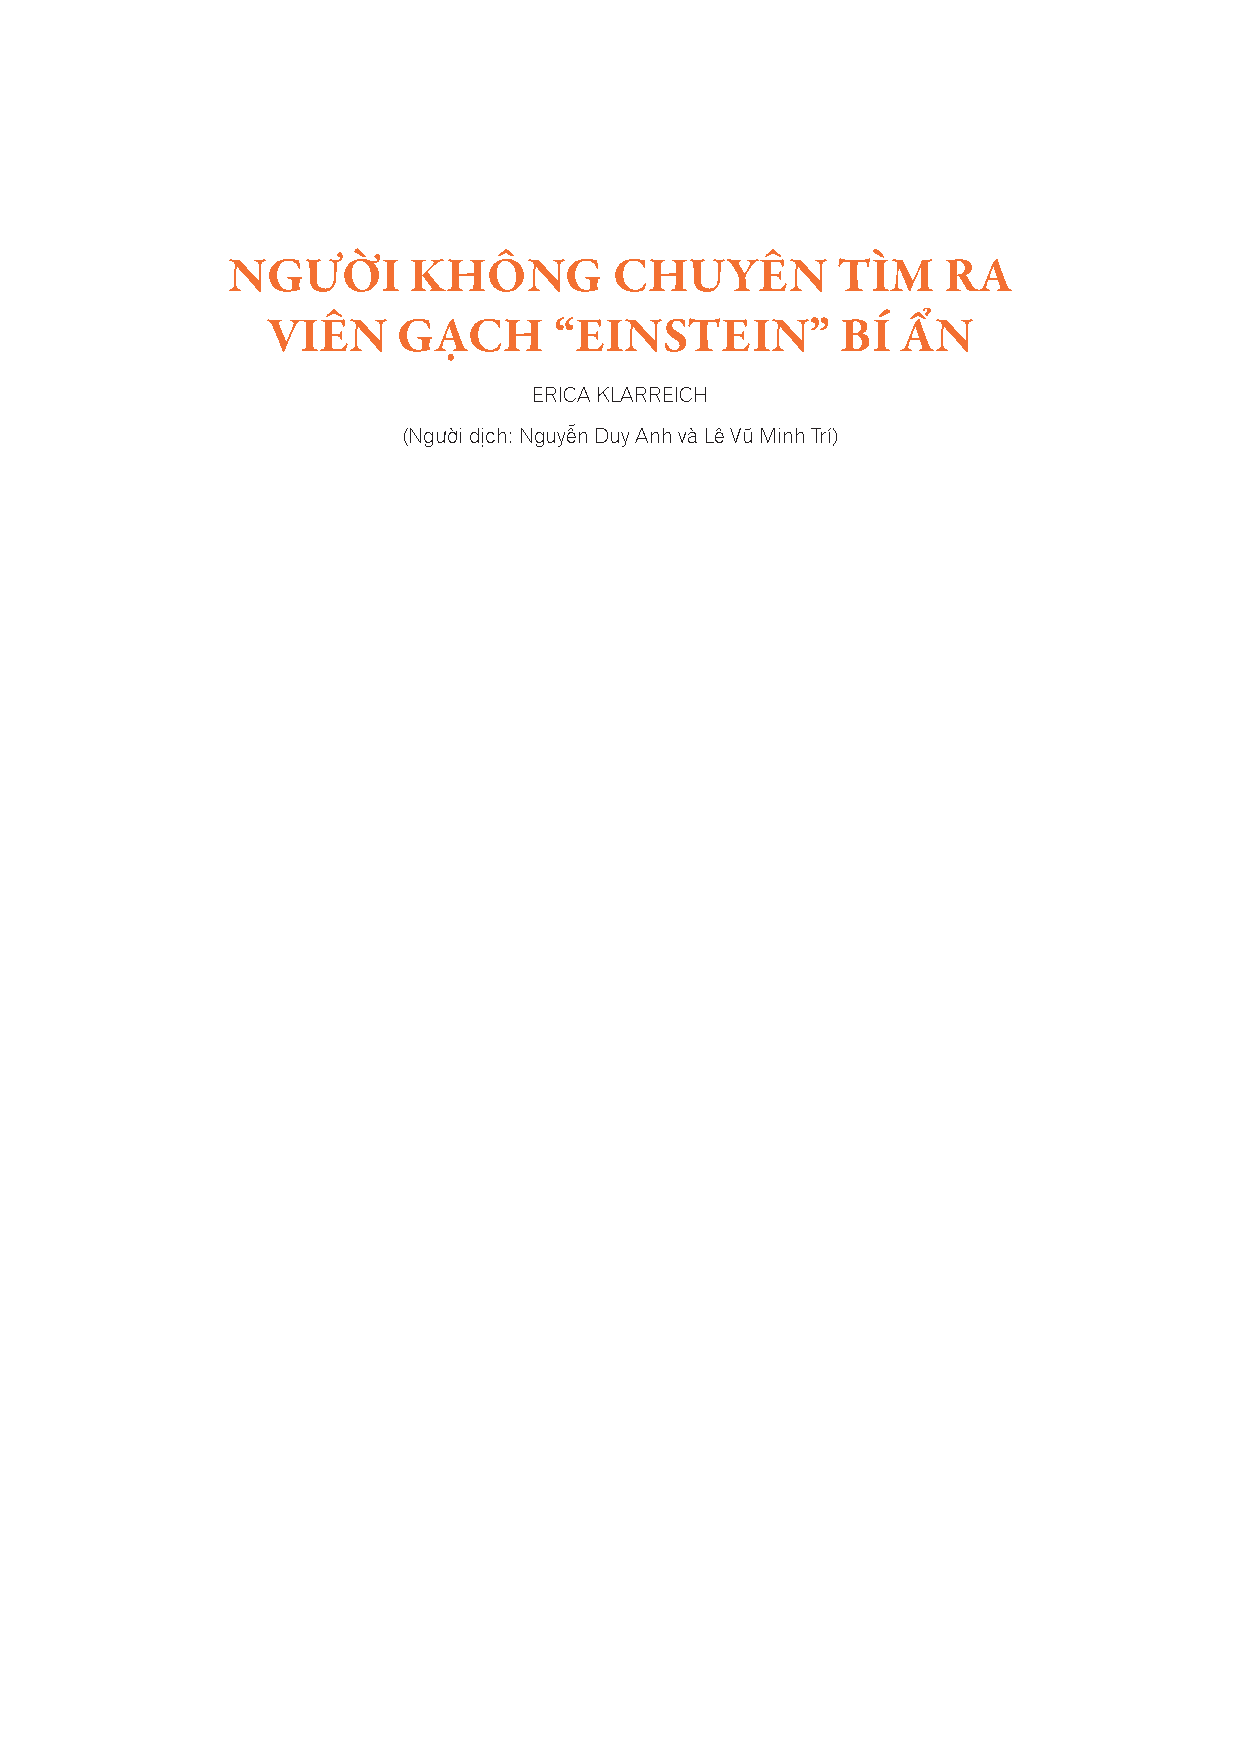
\includegraphics[scale=1]{../tieude1.pdf}}}
\centering
\endgroup
\vspace*{185pt}

\begin{multicols}{2}	
	$\pmb{5.}$ \textbf{\color{duongvaotoanhoc}Ký hiệu của mặt đã trải phẳng. Chứng minh định lý}
	\vskip 0.1cm
	Trải phẳng cho phép chúng ta đưa việc phân loại mặt đóng từ một bài toán tôpô thành một bài toán hình học tổ hợp. Để mô tả một mặt compact đã trải phẳng, ta dùng khái niệm sau đây. Cho $X$ là một mặt compact và xét một trải phẳng của $X$. Đó là một đa giác cong hữu hạn với một số cặp cạnh được dán lại với nhau theo một chiều nào đó. Ta dùng các chữ cái để đặt tên cho các cạnh của đa giác cong sao cho các cạnh được dùng một chữ cái khi và chỉ khi chúng được dán lại với nhau. Ta đánh mũi tên cho các cạnh để thể hiện chiều dán; đối với những cạnh biên (chỉ xuất hiện một lần, không dán với cạnh nào khác) thì ta đánh mũi tên tùy ý. Ta bắt đầu từ một đỉnh tùy ý và lần lượt đi qua các cạnh của đa giác cong theo một chiều xác định trên mặt phẳng (chẳng hạn, ngược chiều kim đồng hồ) và lần lượt viết tên các cạnh thành một dãy theo quy tắc sau: nếu cạnh $a$ cùng chiều với hướng đi đã chọn thì viết $a$, ngược lại thì viết $a^{-1}$. Ta thu được một dãy ký tự, được gọi là một {\it ký hiệu} của mặt $X$.
	\vskip 0.1cm
	Chẳng hạn, mặt cầu có thể được mô tả bởi ký hiệu $aa^{-1}$ hoặc $abb^{-1}a^{-1}$, mặt xuyến có thể được mô tả bởi ký hiệu $aba^{-1}b^{-1}$, mặt phẳng xạ ảnh có thể được mô tả bởi ký hiệu $aa$ hoặc $abab$, chai Klein có thể được mô tả bởi ký hiệu $aba^{-1}b$ (xem các Hình $12$, $14$, $16$ và $18$).
	\vskip 0.1cm
	Ký hiệu cho phép ta mô tả tổng liên thông một cách đơn giản. Thật vậy, giả sử $X, Y$ là các mặt compact, $S_1$ là một ký hiệu của $X$ và $S_2$ là một ký hiệu của $Y$. Ta khoét một đĩa mở $D_1^\circ$ khỏi $X$ sao cho biên $\partial D_1$ đi qua đỉnh đầu (cũng là đỉnh cuối) của đường đi mà ta đã chọn để định nghĩa $S_1$. Mặt thu được được cho bởi ký hiệu $S_1a$, với $a$ là một chữ cái chưa xuất hiện trong $S_1$ (dùng để ký hiệu $\partial D_1$). Khoét một đĩa mở $D_2^\circ$ khỏi $Y$ theo cách tương tự, ta thu được mặt $S_2$ cho bởi ký hiệu $aS_2$. Dán hai mặt vừa thu được theo cạnh $a$, ta thu được tổng liên thông $X \# Y$, được cho bởi ký hiệu $S_1S_2$. Tóm lại, ta chỉ cần viết một ký hiệu của $X$ liền với một ký hiệu của $Y$ để thu được một ký hiệu của $X \# Y$. Chẳng hạn, mặt $\mathbb{T}^{\# g}$ được mô tả bởi ký hiệu $a_1b_1a_1^{-1}b_1^{-1}a_2b_2a_2^{-1}b_2^{-1}\ldots a_gb_ga_g^{-1} b_g^{-1}$, trong khi mặt $\mathbb{P}^{\# g}$ được mô tả bởi ký hiệu $a_1a_1a_2a_2\ldots a_ga_g$.
	\vskip 0.1cm
	Ta bắt đầu chứng minh một nửa của định lý chính bằng cách chỉ ra rằng mọi mặt đóng đều đồng phôi với một trong các mặt $\mathbb{S}$, $\mathbb{T}^{\#g}$ hoặc $\mathbb{P}^{\#g}$ (với $g \ge 1$). Xét $X$ là một mặt đóng. Ta trải phẳng nó, đặt tên và định hướng các cạnh một cách thích hợp. Lúc này, đa giác cong thu được gồm các cặp cạnh (vì $X$ không có biên). Chứng minh được chia thành $4$ bước như sau.
	\vskip 0.1cm
	{\bf\color{duongvaotoanhoc} Bước $\pmb{1.}$ Khử các cặp cạnh kề dạng $\{a,a^{-1}\}$.} Ta có thể giả sử đa giác cong thu được có ít nhất $4$ cạnh, vì nếu nó chỉ có một cặp cạnh thì $X \approx \mathbb{S}$ hoặc $X \approx \mathbb{P}$, tùy theo cách hai cặp cạnh này được dán với nhau (xem Hình $18$). Giả sử có một cặp cạnh kề dạng $\{a,a^{-1}\}$. Ta có thể dán nó lại để khử nó khỏi phép trải phẳng, như trong Hình $25$.
	\begin{figure}[H]
		\vspace*{-5pt}
		\centering\captionsetup{labelformat=empty, justification=centering}
		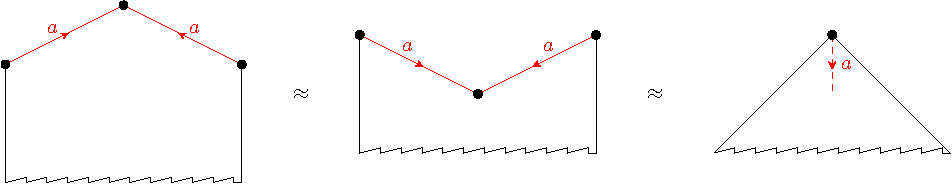
\includegraphics[width=1\linewidth]{H25.pdf}
		\caption{\small\textit{\color{duongvaotoanhoc}Hình $25$: Khử các cặp cạnh kề dạng $\{a,a^{-1}\}$.}}
		\vspace*{-10pt}
	\end{figure}
	Ta lặp lại thao tác khử này cho đến khi $X$ có chỉ còn $2$ cạnh hoặc không còn cặp cạnh kề nào như trên.
	\vskip 0.1cm
	{\bf\color{duongvaotoanhoc} Bước $\pmb{2.}$ Đưa về đa giác cong mà mọi đỉnh đều được dán lại thành một đỉnh.} Đối với mặt xuyến cho bởi ký hiệu $aba^{-1}b^{-1}$, ta thấy rằng $4$ đỉnh của trải phẳng trên được dán lại thành một đỉnh duy nhất. Ta sẽ làm điều này cho mặt đóng $X$ tùy ý. Nếu $x$ là một đỉnh của đa giác cong, ta ký hiệu bởi $[x]$ tập hợp các đỉnh được dán với $x$. Rõ ràng, $[x] = [y]$ nếu $x$ và $y$ được dán với nhau và $[x] \cap [y] = \varnothing$ nếu không.
	\vskip 0.1cm
	Giả sử $x$ và $y$ là hai đỉnh của đa giác cong không được dán với nhau. Ký hiệu bởi $b$ cạnh với hai đầu mút $x,y$, và định hướng lại (nếu cần) sao cho $x$ là điểm cuối của $b$. Ký hiệu bởi $a$ cạnh kề với $b$ tại đầu mút $x$ và gọi $z$ là đầu mút còn lại. Chú ý các cạnh $a$ và $b$ không được dán với nhau (vì nếu vậy thì $x$ phải là điểm cuối của $a$, từ đó ta thu được một cặp cạnh kề nhau dạng $\{a,a^{-1}\}$, mâu thuẫn với giả sử rằng ta đã thực hiện triệt để Bước $1$). Định hướng lại $a$ nếu cần để $x$ là điểm cuối. Ta cắt đa giác cong theo một cạnh $c$ từ $z$ đến $y$, và dán lại dọc theo cạnh $a$. Nếu $[x]$ có ít nhất hai đỉnh thì ở đa giác cong mới thu được, số đỉnh của $[x]$ giảm đi $1$ và số đỉnh của $[y]$ tăng thêm $1$ (xem Hình $26$).
	\begin{figure}[H]
		\vspace*{-5pt}
		\centering\captionsetup{labelformat=empty, justification=centering}
		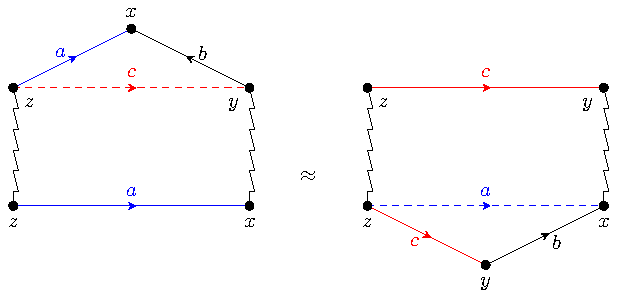
\includegraphics[width=1\linewidth]{H26.pdf}
		\caption{\small\textit{\color{duongvaotoanhoc}Hình $26$: Giảm số đỉnh được dán với $x$ đi 1 và tăng số đỉnh được dán với $y$ thêm $1$.}}
		\vspace*{-10pt}
	\end{figure}
	Ta lặp lại quá trình trên cho đến khi $[x] = \{x\}$. Lúc này, ta thu được một cặp cạnh kề dạng $\{a,a^{-1}\}$ với điểm cuối là $x$ và ta quay lại Bước $1$. Thực hiện phép giản ước ở Bước $1$, ta xóa đỉnh $x$ khỏi đa giác cong, làm giảm tổng số đỉnh (sau khi đã đồng nhất các đỉnh được dán với nhau) đi $1$. Lặp lại toàn bộ quá trình trên (gồm cả Bước $1$ và Bước $2$), sau cùng ta thu được một đa giác cong mà mọi đỉnh đều được dán thành một đỉnh duy nhất.
	\vskip 0.1cm
	{\bf\color{duongvaotoanhoc} Bước $\pmb{3.}$ Thay các cặp cạnh không kề nhau dạng $\{b,b\}$ bởi các cặp cạnh kề nhau.} Giả sử có một cặp cạnh không kề nhau dạng $\{b,b\}$ (dạng $\{b^{-1},b^{-1}\}$ đưa được về dạng này bằng cách định hướng lại). Ta cắt đa giác cong theo một cạnh $a$ nối $2$ điểm cuối của hai cạnh $b$, rồi dán lại dọc theo cạnh $b$ như trong Hình $27$. Chú ý rằng các cặp cạnh kề dạng $\{c,c\}$ hoặc  $\{c^{-1},c^{-1}\}$ (với $c \neq b$) không bị ảnh hưởng bởi thao tác này. Đồng thời, mọi đỉnh vẫn được dán thành một đỉnh duy nhất.
	\begin{figure}[H]
		\vspace*{-5pt}
		\centering\captionsetup{labelformat=empty, justification=centering}
		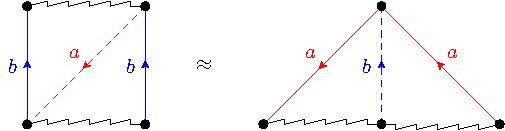
\includegraphics[width=1\linewidth]{H27.pdf}
		\caption{\small\textit{\color{duongvaotoanhoc}Hình $27$: Thay cặp cạnh $\{b,b\}$ bởi cặp cạnh kề nhau $\{a,a\}$.}}
		\vspace*{-10pt}
	\end{figure}
	Lặp lại Bước $3$ cho đến khi mọi cặp cạnh dạng $\{b,b\}$ hoặc $\{b^{-1},b^{-1}\}$ đều kề nhau.
	\vskip 0.1cm
	{\bf\color{duongvaotoanhoc} Bước $\pmb{4.}$ Xử lý các cặp cạnh không kề nhau dạng $\{c,c^{-1}\}$.} Giả sử rằng tồn tại một cặp cạnh không kề nhau dạng $\{c,c^{-1}\}$. Đương nhiên, ta có thể giả sử $c$ là cạnh đầu tiên của đường đi đã chọn, nghĩa là $X$ được cho bởi ký hiệu $cAc^{-1}B$ với $A,B$ là các dãy ký tự khác rỗng. Giả sử phản chứng rằng không có cạnh nào trong $A$ được dán với một cạnh khác trong $B$. Như vậy, các sự dán cạnh chỉ xảy ra trên $A$, trên $B$ hoặc trên cặp $\{c,c^{-1}\}$. Nói riêng, hai đầu mút của $c$ không được dán với nhau, mâu thuẫn với giả thiết rằng mọi đỉnh đã được dán thành một đỉnh duy nhất. Vậy giả sử phản chứng là sai, nghĩa là có một cạnh của $A$ được dán với một cạnh khác trong $B$. Vì các cặp cạnh dạng $\{a,a\}$ đều đã đưa về kề nhau, nên có một cạnh $d$ trong $A$ được dán với cạnh $d^{-1}$ trong $B$, nghĩa là $X$ cho bởi ký hiệu dạng $c\ldots d \ldots c^{-1} \ldots d^{-1}$. Ta thực hiện cắt dán như ở Hình $28$ để thay $2$ cặp $\{c,c^{-1}\}$ và $\{d,d^{-1}\}$ bởi dãy $efe^{-1}f^{-1}$. Chú ý rằng các cặp cạnh kề nhau không bị ảnh hưởng bởi thao tác này. Đồng thời, mọi đỉnh vẫn được dán thành một đỉnh duy nhất.
	\begin{figure}[H]
		\vspace*{-5pt}
		\centering\captionsetup{labelformat=empty, justification=centering}
		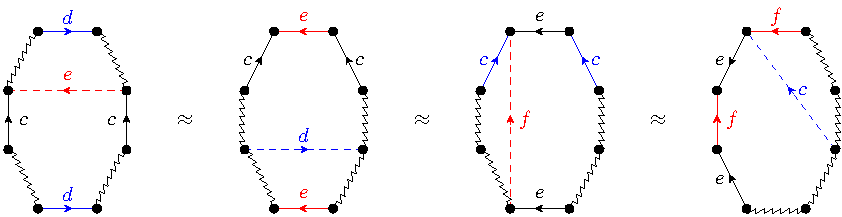
\includegraphics[width=1\linewidth]{H28.pdf}
		\caption{\small\textit{\color{duongvaotoanhoc}Hình $28$: Thay $2$ cặp cạnh $\{c,c^{-1}\}$ và $\{d,d^{-1}\}$ bởi dãy $efe^{-1}f^{-1}$.}}
		\vspace*{-10pt}
	\end{figure}
	Lặp lại Bước $4$ cho đến khi các cặp cạnh dạng $\{c,c^{-1}\}$ được phân hoạch vào cách dãy dạng $efe^{-1}f^{-1}$ (các cặp cạnh dạng $\{b,b\}$ vẫn luôn kề nhau). Ký hiệu thu được mô tả tổng liên thông của một số hữu hạn các mặt xuyến và các mặt phẳng xạ ảnh (mặt xuyến có ký hiệu là $aba^{-1}b^{-1}$ và mặt phẳng xạ ảnh có ký hiệu là $aa$. Vì tính giao hoán của tổng liên thông, ta có $X \approx \mathbb{T}^{\# m} \# \mathbb{P}^{\# n}$, với $m,n \in \mathbb{N}$. Nếu $m=0$ hoặc $n = 0$ thì chứng minh kết thúc. Trong trường hợp $m,n > 0$, ta áp dụng kết quả $\mathbb{T} \# \mathbb{P} \approx \mathbb{P}^3$ (ở cuối mục trước) $m$ lần liên tiếp để thu được $X \approx \mathbb{P}^{\# (2m + n)}$.
	\vskip 0.1cm
	Để chứng minh phần ``duy nhất'' của định lý chính, ta cần chỉ ra rằng các mặt đã liệt kê đôi một không đồng phôi. Một việc có thể làm ngay lúc này là chỉ ra rằng các mặt $\mathbb{P}^{\# g}$ (với $g > 0$) không đồng phôi với các mặt $\mathbb{T}^{\# h}$ (với $h \ge 0$, nhắc lại rằng $\mathbb{T}^0 := \mathbb{S}$). Thật vậy, mặt cầu và mặt xuyến là mặt một phía là các mặt hai phía (vì thế, các mặt xuyến với $h$ quai cầm, $h > 0$, cũng vậy) nên ta chỉ cần chỉ ra rằng rằng $\mathbb{P}^{\# g}$ là mặt một phía với mọi $g > 0$. Thật vậy
	\vskip 0.1cm
	$\bullet$ với $g = 1,2$, ta biết rằng $\mathbb{P}$ và $\mathbb{P} \# \mathbb{P} \approx \mathbb{K}$ (xem Hình $19$) là các mặt một phía, vì chúng đều chứa băng M\"obius (xem Hình $17$);
	\vskip 0.1cm
	$\bullet$ với $g \ge 3$ và chẵn thì $g = 2n$ (với $n \ge 2$), áp dụng liên tiếp kết quả $\mathbb{P}^{\# 3} \approx \mathbb{T} \# \mathbb{P}$, ta có $\mathbb{P}^{\# 2n} \approx \mathbb{T}^{n-1} \# \mathbb{P}^{\# 2} \approx \mathbb{T}^{n-1} \# \mathbb{K}$ là mặt một phía (vì $\mathbb{T}^{n-1}$ là mặt hai phía còn $\mathbb{K}$ là mặt một phía);
	\vskip 0.1cm	
	$\bullet$ với $g \ge 3$ và lẻ thì $g = 2n+1$ (với $n \ge 1$), tương tự, ta có $\mathbb{P}^{\#(2n+1)} \approx \mathbb{T}^n \# \mathbb{P}$ là mặt một phía (vì $\mathbb{T}^{n}$ là mặt hai phía còn $\mathbb{P}$ là mặt một phía).
	\vskip 0.1cm
	Phần còn lại của chứng minh cho tính duy nhất sẽ được hoãn lại tới mục sau, nơi ta giới thiệu thêm một bất biến tôpô quan trọng khác.
	\vskip 0.1cm
	$\pmb{6.}$ \textbf{\color{duongvaotoanhoc}Đặc trưng Euler--Poincar\'e. Giống}
	\vskip 0.1cm
	Cho $X$ là một mặt đóng và $\mathscr{T}$ là một phép tam giác phân hữu hạn của $X$. Lần lượt ký hiệu bởi $V(\mathscr{T})$, $E(\mathscr{T})$ và $F(\mathscr{T})$ số đỉnh, số cạnh và số tam giác cong trong $\mathscr{T}$. Số nguyên
	\begin{align*}
		\chi(\mathscr{T}) = V(\mathscr{T}) - E(\mathscr{T}) + F(\mathscr{T})
	\end{align*}
	là {\it đặc trưng Euler--Poincar\'e} của $\mathscr{T}$. Ta sẽ dùng giá trị này để chỉ ra rằng $\mathbb{S}$ không đồng phôi với $\mathbb{T}^m$ với $m > 0$ và rằng $\mathbb{T}^m$ không đồng phôi với $\mathbb{T}^n$ cũng như $\mathbb{P}^m$ không đồng phôi với $\mathbb{P}^n$ với $m \neq n$. Trước hết, ta cần chỉ ra rằng giá trị $\chi$ là một bất biến tôpô chỉ phụ thuộc vào nội tại mặt $X$, không phụ vào phép tam giác phân $\mathscr{T}$. Trong tôpô đại số, điều này được chứng minh nhờ khái niệm {\it lý thuyết đồng điều} và một tính toán đơn giản trên các {\it số Betti}. 
	\vskip 0.1cm
	Ở mục này, chúng ta cố gắng phác thảo một chứng minh không chính thức cho sự kiện này. Ý tưởng như sau, cho $\mathscr{T}$ và $\mathscr{T}'$ là hai tam giác phân tùy ý, ta dùng một số hữu hạn các phép biến đổi bảo toàn đặc trưng Euler--Poincar\'e để đưa $\mathscr{T}$ về $\mathscr{T}'$. Để làm điều này một cách thuận tiện, ta đưa ra một khái niệm tổng quát hơn tam giác phân: Ta gọi một {\it cấu trúc phân ngăn} trên $X$ là một họ $\mathscr{C}$ gồm một số hữu hạn các điểm, các đường và các đa giác cong trên $X$, thỏa mãn các tính chất sau.
	\vskip 0.1cm
	$\bullet$ Phần trong của mỗi đa giác cong đều đồng phôi với đĩa mở $\mathbb{D}$ và đôi một không giao nhau.
	\vskip 0.1cm
	$\bullet$ Biên của mỗi đa giác cong là hợp của một số hữu hạn các đường (ta gọi các đường này là các {\it cạnh} của đa giác cong, các đầu mút của chúng là các {\it đỉnh} của đa giác cong).
	\vskip 0.1cm
	$\bullet$ Sau khi bỏ điểm đầu và điểm cuối, các đường đều đồng phôi với khoảng mở $(0,1)$ và đôi một không giao nhau.
	\vskip 0.1cm
	Khái niệm trên cho phép sự xuất hiện của các đường với điểm đầu trùng với điểm cuối (các {\it khuyên}), các đa giác có thể có số cạnh tùy ý (thậm chí có thể bằng $1$ hoặc $2$), xem Hình $29$.
	\begin{figure}[H]
		\vspace*{-5pt}
		\centering\captionsetup{labelformat=empty, justification=centering}
		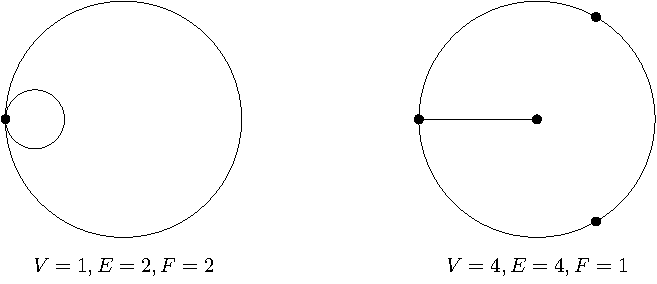
\includegraphics[width=1\linewidth]{H29.pdf}
		\caption{\small\textit{\color{duongvaotoanhoc}Hình $29$: Hai cấu trúc phân ngăn khác nhau của đĩa đóng.}}
		\vspace*{-10pt}
	\end{figure}
	Lần lượt ký hiệu bởi $V(\mathscr{C})$, $E(\mathscr{C})$ và $F(\mathscr{C})$ số điểm, số đường và số đa giác cong trong $\mathscr{C}$. Gọi
	\begin{align*}
		\chi(\mathscr{C}) = V(\mathscr{C}) - E(\mathscr{C}) + F(\mathscr{C})
	\end{align*}
	là đặc trưng Euler--Poincar\'e của $\mathscr{C}$. Dễ thấy các thao tác sau đây không làm thay đổi đặc trưng Euler--Poincar\'e của cấu trúc phân ngăn.
	\vskip 0.1cm
	$\bullet$ Chia đôi một đường bằng cách thêm một điểm vào giữa đường (số điểm và số đường đều tăng thêm $1$, số đa giác cong không đổi).
	\vskip 0.1cm	
	$\bullet$ Chia đôi một đa giác cong bằng cách thêm một đường nối hai đỉnh {\it không nhất thiết phân biệt} (số điểm không đổi, số đường và số đa giác cong đều tăng thêm $1$).
	\vskip 0.1cm	
	$\bullet$ Thêm một điểm ở miền trong của một đa giác cong và một đường nối nó với một đỉnh của đa giác (số điểm và số đường đều tăng thêm $1$, số đa giác cong không đổi).
	\vskip 0.1cm
	Giả sử $\mathscr{C}$ và $\mathscr{C}'$ là hai cấu trúc phân ngăn sao sao cho giao của mỗi đường của $\mathscr{C}$ với mỗi đường của $\mathscr{C}'$ chỉ gồm một số hữu hạn các điểm và một số hữu hạn các đoạn đóng. Khi đó ta có thể dùng một số hữu hạn các phép biến đổi trên để đưa $\mathscr{C}$ và $\mathscr{C}'$ về cùng một cấu trúc phân ngăn $\mathscr{C}''$, chẳng hạn như trong Hình $30$. Vì thế, ta có $\chi(\mathscr{C}) = \chi(\mathscr{C}'') = \chi(\mathscr{C}')$.
	\begin{figure}[H]
		\vspace*{-5pt}
		\centering\captionsetup{labelformat=empty, justification=centering}
		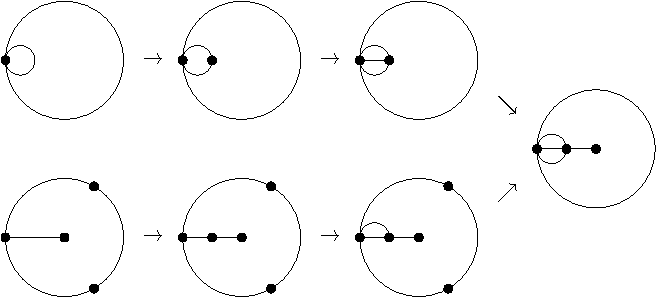
\includegraphics[width=1\linewidth]{H30.pdf}
		\caption{\small\textit{\color{duongvaotoanhoc}Hình $30$: Đưa hai cấu trúc phân ngăn ở Hình $29$ về cùng một cấu trúc phân ngăn.}}
		\vspace*{-10pt}
	\end{figure}
	Trường hợp xấu có thể xảy ra là khi giao của một đường trong $\mathscr{C}$ với một đường trong $\mathscr{C}'$ gồm một số vô hạn điểm hoặc một số vô hạn đoạn đóng. Lúc này, ta cần ``xê dịch'' hai đường này một chút để đưa về trường hợp trước. Đây là một bước rất kỹ thuật và cần dùng đến tính compact trong tôpô học, ta sẽ không đi sâu vào chi tiết.
	\vskip 0.1cm
	Từ các phân tích ở trên, ta có thể định nghĩa đặc trưng Euler--Poincar\'e $\chi(X)$ của một mặt đóng $X$ là đặc trưng Euler--Poincar\'e $\chi(\mathscr{T})$ của bất kỳ phép tam giác phân hữu hạn $\mathscr{T}$ (hoặc bất kỳ cấu trúc phân ngăn hữu hạn $\mathscr{C}$) nào của $X$. Chẳng hạn, mặt xuyến có một tam giác phân $\mathscr{T}$ cho bởi Hình $13$, với $V(\mathscr{T}) = 9$, $E(\mathscr{T}) = 27$ và $F(\mathscr{T}) = 18$, nên $\chi(\mathbb{T}) = 9 - 27 + 18 = 0$. Một phép đồng phôi biến một tam giác phân của mặt này thành một tam giác phân của mặt kia, với số đỉnh, số cạnh và số tam giác cong được bảo toàn. Vì thế, hai mặt đồng phôi có cùng đặc trưng Euler--Poincar\'e, nghĩa là đặc trưng Euler--Poincar\'e là một bất biến tôpô.
	\vskip 0.1cm
	Cho $X$ và $Y$ là các mặt đóng, ta tìm công thức liên hệ giữa $\chi(X \# Y)$ với $\chi(X)$ và $\chi(Y)$ như sau. Xét $\mathscr{T},\mathscr{T}'$ lần lượt là các tam giác phân hữu hạn bất kỳ của $X$ sao cho có ít nhất một tam giác cong $T \in \mathscr{T}$ nằm trong $X^\circ$ và ít nhất một tam giác cong $T' \in \mathscr{T}'$ nằm trong $Y^\circ$. Ta khoét $T^{\circ}$ và $T'^{\circ}$ khỏi $X$ và $Y$ rồi dán $X \setminus T^\circ$ với $Y \setminus T'^{\circ}$ dọc theo $\partial T \approx \partial T'$ để thu được tổng liên thông $X \# Y$. Có $3$ đỉnh được dán lại với nhau, $3$ cạnh được dán lại với nhau, và $2$ tam giác cong bị bỏ đi, do đó tam giác phân mới thu được trên $X\#Y$ gồm $V(\mathscr{T}) + V(\mathscr{T}') - 3$ đỉnh, $E(\mathscr{T}) + E(\mathscr{T}') - 3$ cạnh và $F(\mathscr{T}) + F(\mathscr{T}') - 2$ tam giác cong. Từ đó ta tính được
	\begin{align*}
		\chi(X \# Y) = \chi(X) + \chi(Y) - 2.
	\end{align*}
	Thay $Y = \mathbb{S}$ trong công thức trên (nhắc lại rằng $X \# \mathbb{S} \approx X$), ta thu được $\chi(\mathbb{S}) = 2$. Mặt khác, bằng quy nạp, ta dễ dàng tính được
	\begin{align*}
		\chi(X^{\# g}) = g \cdot \chi(X) + 2 - 2g
	\end{align*}
	với $g \ge 1$. Từ đó ta có $\chi(\mathbb{T}^{\# g}) = 2-2g \le 0$. Do đó, mặt $\mathbb{S}$ cùng các mặt $\mathbb{T}^g$, với $g \ge 1$, đôi một không đồng phôi (nhắc lại rằng tất cả các mặt này đều là mặt hai phía).
	\vskip 0.1cm
	Ngoài ra, từ kết quả $\mathbb{P} \# \mathbb{T} \approx \mathbb{P}^{\# 3}$, ta tính được $\chi(\mathbb{P}) = 1$, suy ra $\chi(\mathbb{T}^{\# g}) = 2-g$. Do đó, các mặt $\mathbb{P}^g$, với $g \ge 1$, đôi một không đồng phôi (nhắc lại rằng tất cả các mặt này đều là mặt một phía). Điều này kết thúc chứng minh của định lý phân loại tôpô cho các mặt đóng.
	\vskip 0.1cm
	Ta kết thúc bài viết bằng việc nhắc đến khái niệm sau đây. Với $X$ là một mặt đóng, nếu $X$ là mặt hai phía thì tồn tại duy nhất số tự nhiên $g$ sao cho $\chi(X) = 2-2g$, hay $X \approx \mathbb{T}^{\#g}$ (nhắc lại quy ước $\mathbb{T}^{\# 0} = \mathbb{S}$). Số tự nhiên $g$ này được gọi là {\it giống} (genus) của mặt $X$, nó chính là ``số quai cầm'' của $X$ (mặt cầu không có quai cầm, tổng liên thông $\mathbb{T}^{\# g}$ có $g$ quai cầm). Theo tinh thần này, nếu $X$ là mặt một phía thì tồn tại duy nhất số nguyên dương $g$ sao cho $\chi(X) = 2-g$ (ta có $X \approx \mathbb{P}^{\# g}$). Ta cũng gọi $g$ là giống của $X$ trong trường hợp này (một số nơi gọi số nguyên này là {\it á giống}). Định lý chính của bài viết này nói rằng, mặt đóng $X$ được xác định duy nhất (sai khác đồng phôi) khi ta biết tính khả định hướng và giống của nó.
\end{multicols}
\vspace*{-10pt}
{\color{duongvaotoanhoc}\rule{1\linewidth}{1pt}}
\vskip 0.2cm
\centerline{\Large{\textbf{\color{duongvaotoanhoc}LỜI GIẢI, ĐÁP ÁN}}}
\vskip 0.1cm
\begin{multicols}{2}
	\textbf{\color{duongvaotoanhoc}Một bộ tộc kỳ lạ}
	\vskip 0.1cm
	Ta sẽ gọi chung những người Thật thà và những người Nói dối của bộ tộc đó là những người sống theo nguyên tắc. Tiếp theo ta có $2$ cách lập luận.
	\vskip 0.1cm
	\textit{Cách $1$}: 
	Có $250$ câu trả lời ``Có", $250$ câu trả lời ``Không". Mỗi một người Phụ hoạ không thể làm tăng số câu trả lời thiểu số trong số ``Có" hoặc ``Không" tính đến trước anh ta, trong khi người ``nguyên tắc" mới tạo ra sự thay đổi của số số câu trả lời thiểu số này. Do số câu trả lời thiểu số tăng dần từ $0$ tới $250$, và với mỗi một câu trả lời mới, số câu trả lời thiểu số thay đổi không quá $1$, nên số những người sống theo nguyên tắc của bộ tộc phải ít nhất là $250$ người. Do đó số người Phụ hoạ tối đa là $250$ người.
	\vskip 0.1cm
	\hfill \textit{(Xem tiếp trang $56$)}
\end{multicols}